前几节描述了传递给parallel\_for的参数,如何影响内核分配给GPU资源,以及在GPU上执行内核所涉及的软件层和开销。本节介绍了内核在GPU上执行的最佳实践。\par

内核要么是内存式的,其性能受到数据读写操作在GPU上执行资源的限制,要么是计算式的,其的性能受到GPU上执行资源的限制。这是为GPU和许多其他处理器优化内核的良好第一步!——用来确定内核是内存式,还是计算式的,因为改进内存式内核的技术通常不会有益于计算式内核,反之亦然。所以供应商通常提供分析工具来帮助确定。\par

\begin{tcolorbox}[colback=red!5!white,colframe=red!75!black]
需要不同的优化技术,这取决于内核是内存式还是计算式!
\end{tcolorbox}

因为GPU倾向于拥有许多处理器和较宽的SIMD,内核倾向于内存式,而不是计算式。如果不确定从哪里开始,检查内核如何访问内存是很好的一步。\par

\hspace*{\fill} \par %插入空行
\textbf{访问全局内存}

高效地访问全局内存对于优化应用程序性能至关重要,因为工作项或工作组操作的几乎所有数据都源自全局内存。当内核在全局内存上的操作效率很低,那性能会很差。尽管GPU通常包含专用硬件集合和计算单元,用于读写内存中的任意位置,但访问全局内存的性能通常是由数据访问的局域性驱动。当工作组中的工作项正在访问内存中的一个元素,该元素与工作组中另一个工作项访问的元素相邻,则全局内存访问性能可能会很好。如果工作组中的工作项访问的内存是跨步的或随机的,则全局内存访问性能会差。一些GPU文档将附近内存访问操作描述为\textbf{合并访问}。\par

在图15-15中某种程度上并行的矩阵乘法内核,可以选择是并行处理一行还是一列,这里选择并行处理结果矩阵的行。这是一个糟糕的选择:如果一个id等于m的工作项与一个id等于m-1或m+1的相邻工作项分组,用于访问matrixB的索引对于每个工作项都是相同的,但是用于访问matrixA的索引不同于K,这意味着访问是高度跨步的。matrixA的访问模式如图15-17所示。\par

\hspace*{\fill} \par %插入空行
图15-17 对matrixA的访问是高度跨越和低效的
\begin{center}
	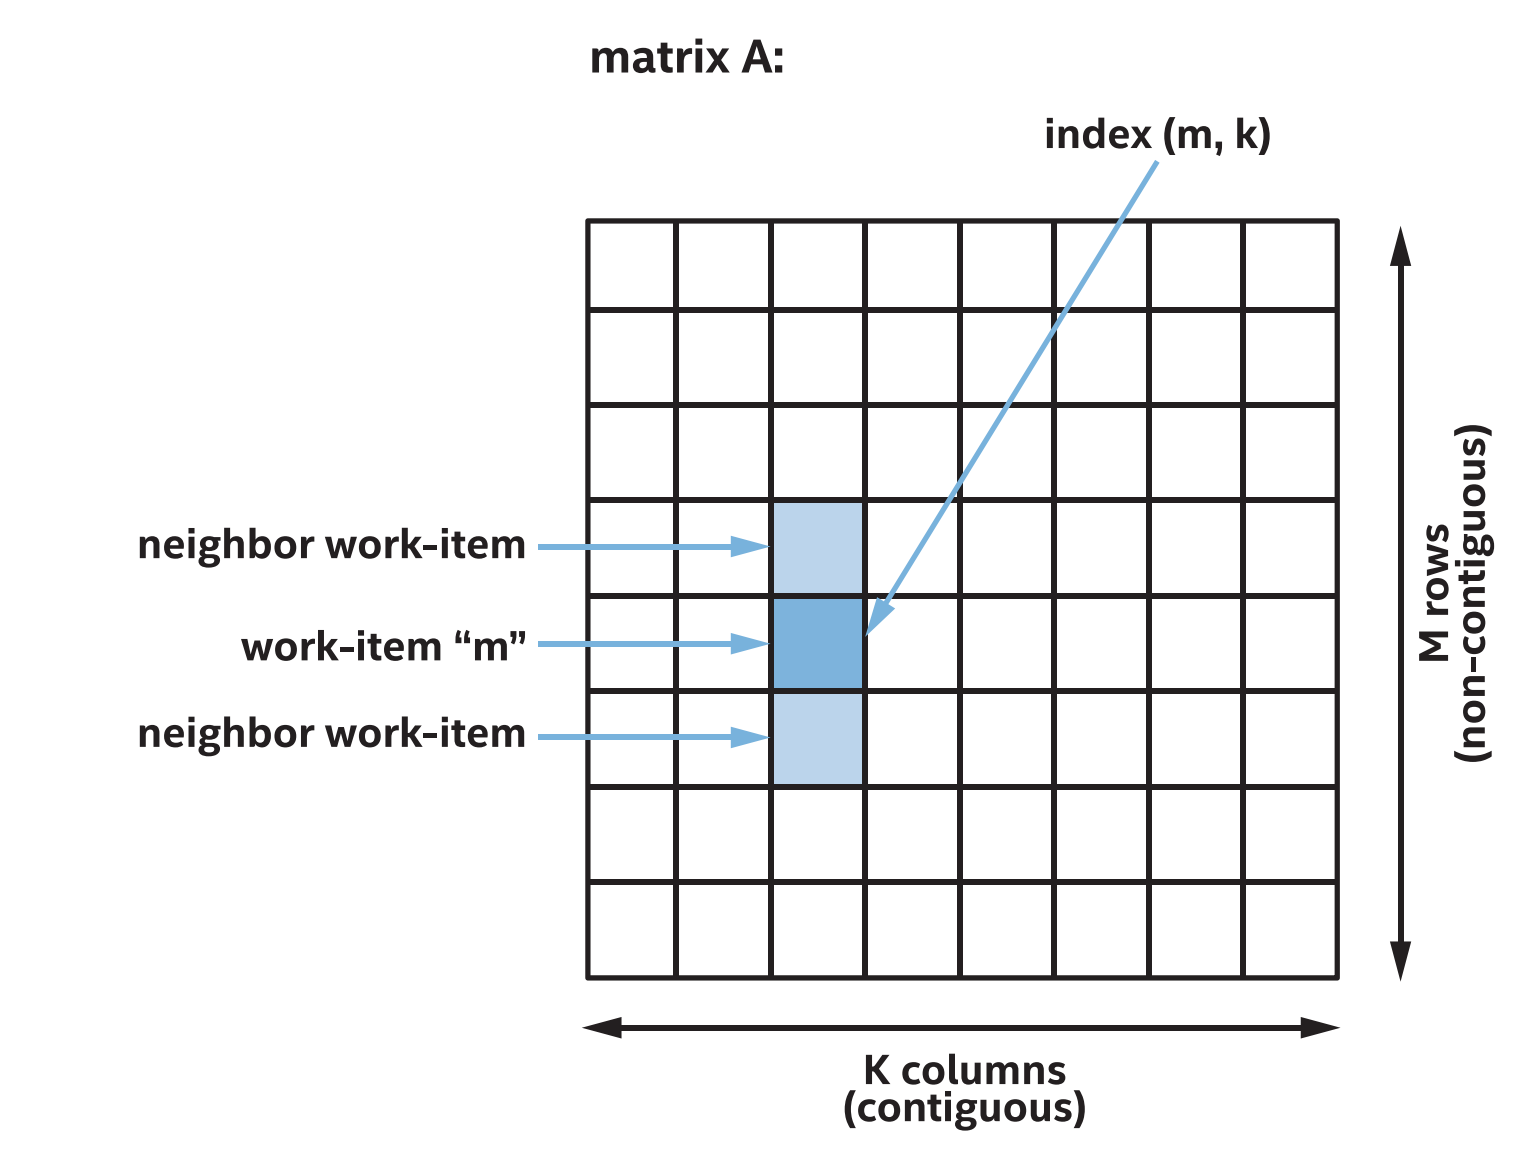
\includegraphics[width=0.8\textwidth]{content/chapter-15/images/13}
\end{center}

如果选择并行处理结果矩阵的列,则访问模式具有更好的局部性。图15-18中的内核在结构上与图15-5中相似,唯一的区别是图15-18中的每个工作项操作的是结果矩阵的一列,而不是结果矩阵的一行。\par

\hspace*{\fill} \par %插入空行
图15-18 并行计算结果矩阵的列,而不是行
\begin{lstlisting}[caption={}]
// This kernel processes columns of the result matrix in parallel.
h.parallel_for(N, [=](item<1> idx) {
	int n = idx[0];
	
	for (int m = 0; m < M; m++) {
		T sum = 0;
		for (int k = 0; k < K; k++)
			sum += matrixA[m * K + k] * matrixB[k * N + n];
		matrixC[m * N + n] = sum;
	}
});
\end{lstlisting}

尽管这两个内核在结构上非常相似,但在许多GPU上操作数据列的内核将显著优于操作数据行的内核,纯粹是因为更高效的内存访问:如果一个id等于n的工作项与一个id等于n-1或n+1的相邻工作项分组,用于访问matrixA的索引现在对于每个工作项都是相同的,并且用于访问matrixB的索引是连续的。matrixB的访问模式如图15-19所示。\par

\hspace*{\fill} \par %插入空行
图15-19 对matrixB的访问是连续的和有效的
\begin{center}
	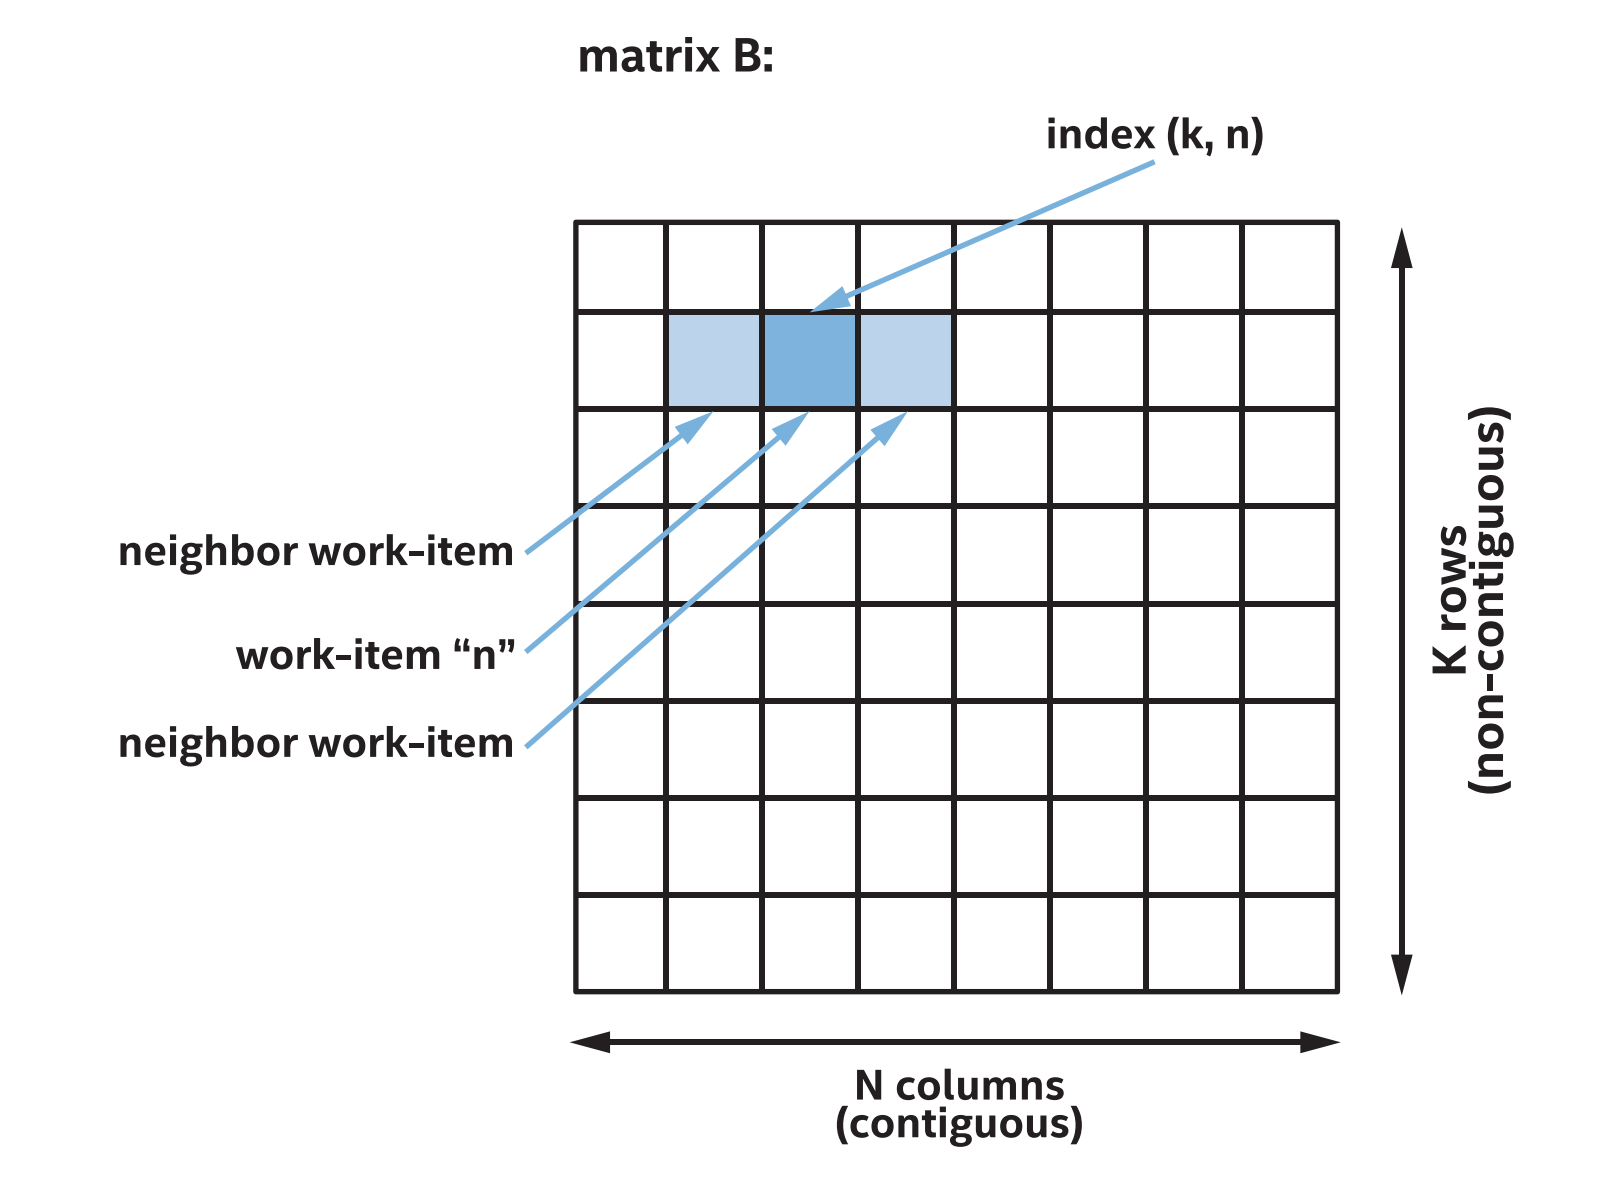
\includegraphics[width=0.8\textwidth]{content/chapter-15/images/14}
\end{center}

对连续数据的访问通常非常有效。根据经验,访问一组工作项的全局内存的性能取决于访问的GPU缓存行的数量有访问都在一个缓存行内,访问将以最高性能执行。一个访问需要两条缓存线,比如通过访问每个其他元素或者从缓存不对齐的地址开始,访问可能会以一半的性能运行。组中的每个工作项访问唯一的高速缓存行,例如:对于非常频繁的或随机的访问,就可能以最低的性能运行。\par

\begin{tcolorbox}[colback=blue!5!white,colframe=blue!75!black, title=设置内核变体]
对于矩阵乘法,选择沿着一个维度并行化,显然可以提高内存访问效率,但对于其他内核,选择可能不那么明显。在实现最佳性能非常重要的内核中,如果不清楚并行化的维度,那么有时值得开发和分析沿每个维度并行化的不同内核变体,以了解哪种方法更适合设备和数据集。
\end{tcolorbox}

\hspace*{\fill} \par %插入空行
\textbf{访问工作组本地内存}

前一节中,我们描述了对全局内存的访问如何从局部性中获益,从而最大化缓存性能。某些情况下,可以设计算法来有效地访问内存,比如选择在一个维度上并行化。然而,并非所有情况下都能使用这种技术。本节描述如何使用工作组本地内存来有效地支持更多的内存访问模式。\par

从第9章开始,工作组中的工作项可以通过工作组本地内存通信和使用工作组栅栏同步来协作解决问题。这种技术对GPU有利,因为典型的GPU有专属硬件来实现栅栏和工作组本地内存。不同的GPU厂商和不同的产品可能会以不同的方式实现工作组本地内存,但是工作组本地内存与全局内存相比通常有两个优势:本地存储器可以支持比对全局存储器的访问更高的带宽和更低的等待时间,即使当全局存储器访问命中高速缓存时,并且本地存储器通常被划分为不同的存储器区域,称为存储库。只要组中的每个工作项访问不同的存储库,本地内存访问就会以完全的性能执行。存储库访问允许本地存储器支持比全局存储器更多的具有峰值性能的访问模式。\par

许多GPU供应商会将连续的本地内存地址分配给不同的存储地址。这确保了连续的内存访问总是完全的性能操作,而不管起始地址是什么。但当内存访问是有跨距访问时,组中的一些工作项可能访问分配给同一存储地址。当发生这种情况时,认为是存储地址冲突,从而导致序列化访问和较低的性能。\par

\begin{tcolorbox}[colback=red!5!white,colframe=red!75!black]
为了获得最大的全局内存性能,应尽量减少访问的高速缓存行的数量。\\

为了获得最大的本地内存性能,尽量减少内存地址冲突!
\end{tcolorbox}

图15-20概述了全局内存和本地内存的访问模式和预期性能。假设当ptr指向全局内存时,指针与GPU缓存行的大小对齐。访问全局内存时,可以通过从缓存对齐的地址连续访问内存来获得最佳性能。访问未对齐的地址可能会降低全局内存性能,因为访问可能需要访问额外的缓存行。因为访问未对齐的本地地址不会导致存储地址冲突,所以本地内存性能没有改变。\par

有跨距的案例值得更详细地描述。访问全局内存中的每一个元素都需要访问更多的缓存行,这可能会导致较低的性能。访问本地内存中的每一个元素可能会导致存储地址冲突和性能下降,但只有当存储地址的块数量能被2整除时。如果存储地址块的数量是奇数,这种情况也将全速运行。\par

当访问之间的跨越非常大时,每个工作项访问唯一的缓存行,从而导致最差的性能。但是对于本地内存,性能取决于步幅和存储地址块的数量。当步长N等于存储地址块数量时,每次访问都会导致内存块冲突,所有访问都会序列化,导致性能最差。但是,如果步数M和内存块数量没有关系,则访问将以全速运行。因此,许多优化的GPU内核会在本地内存中填充数据结构,以选择减少或消除内存块冲突的方法。\par

\hspace*{\fill} \par %插入空行
图15-20 对于不同的访问模式,全局和本地内存可能的性能情况
\begin{center}
	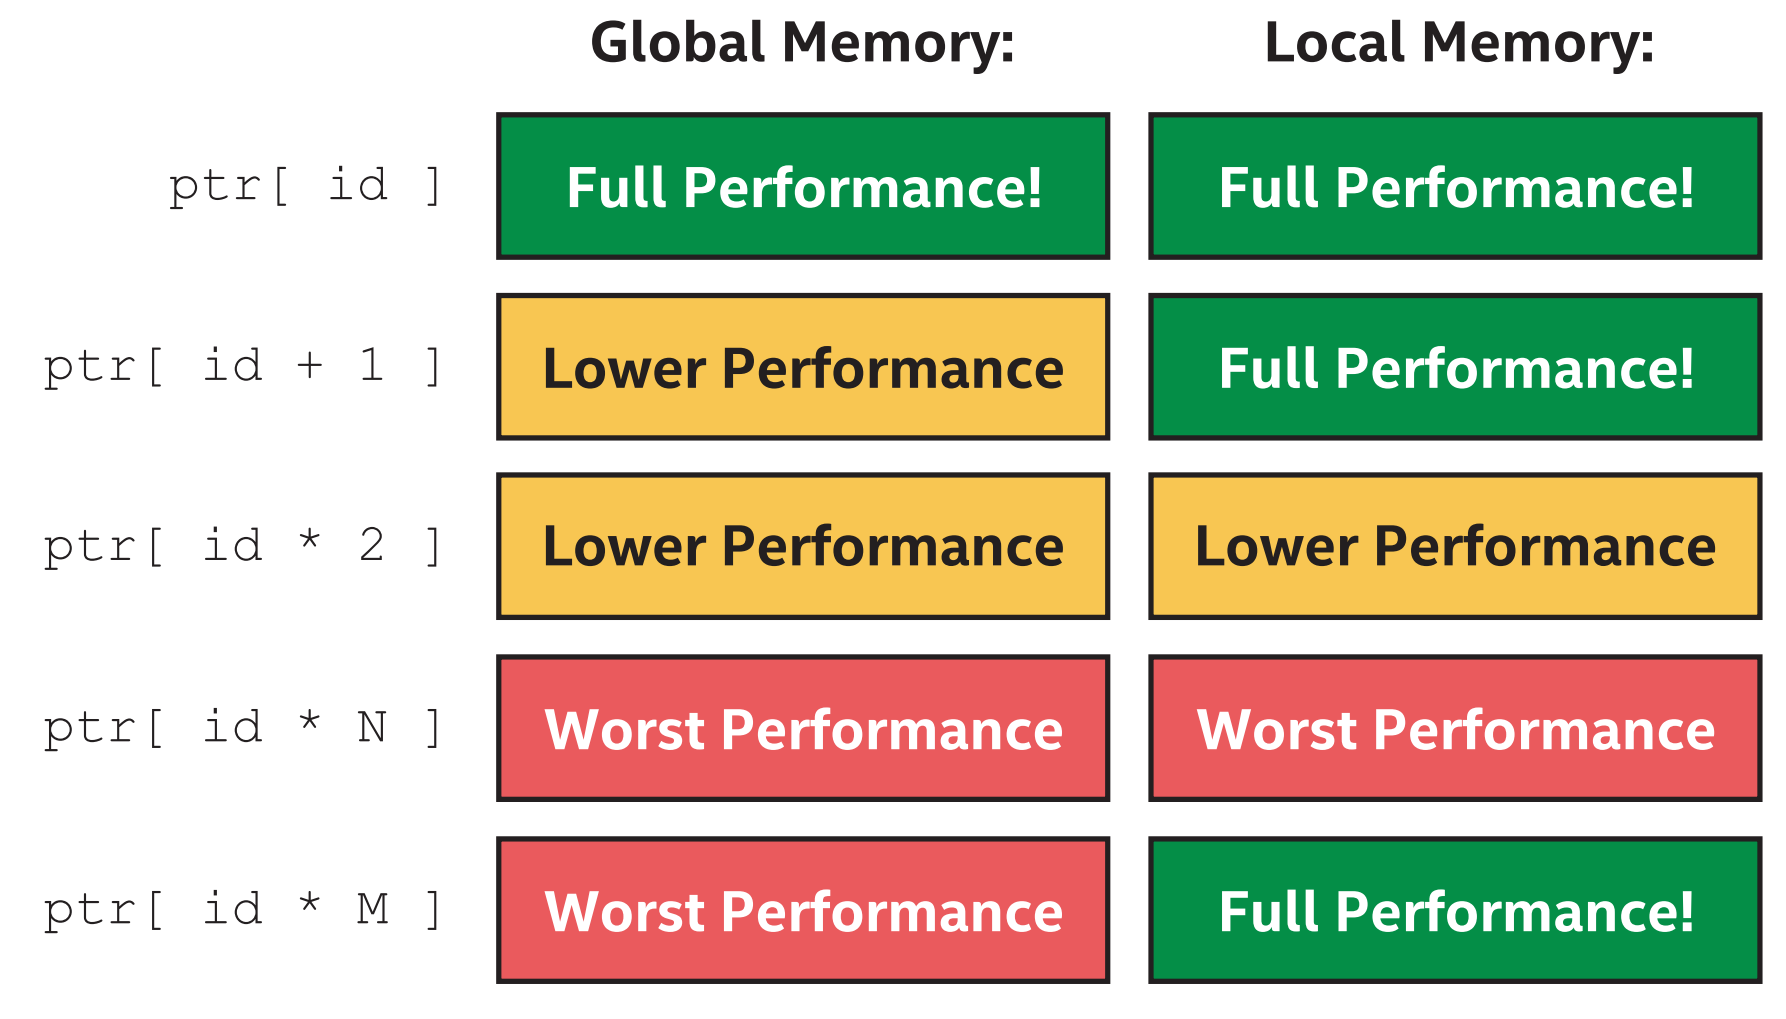
\includegraphics[width=0.8\textwidth]{content/chapter-15/images/15}
\end{center}

\hspace*{\fill} \par %插入空行
\textbf{子工作组不使用本地内存}

正如第9章所讨论的,子工作组集合功能是在组中的工作项之间交换数据的一种替代方法。对于许多GPU,子工作组代表由单个指令流处理的工作项集合。这些情况下,子工作组中的工作项可以在不使用工作组本地内存的情况下,低成本地交换数据和同步。许多性能好的GPU内核都使用子工作组,所以对于内核,我们的算法是否可以重新定义,为使用子工作组集合函数是值得研究的课题。\par

\hspace*{\fill} \par %插入空行
\textbf{使用小数据类型优化计算}

本节描述消除或减少内存访问瓶颈后优化内核的技术。记住,GPU以前是用来在屏幕上绘制图片的。尽管GPU的纯计算能力随着时间的推移不断发展和改进,但在传统的图形学领域能力优势仍然很明显。\par

例如,考虑对内核数据类型的支持。许多GPU都为32位浮点操作进行了高度优化,因为这些操作在图像和游戏中很常见。对于处理较低精度的算法,许多GPU还支持较低精度的16位浮点型,以精度换取更快的处理速度。相反,尽管许多GPU支持64位双精度浮点操作,但高精度是有代价的,32位操作通常比64位操作执行得更快。\par

整数类型也是如此,32位整数数据类型通常比64位整数数据类型执行得更好,而16位整数可能执行得更好。如果可以用更小的整数来组织计算,那么内核可能会执行得更快。特别需要注意的是寻址操作,这些操作通常在64位的size\_t数据类型上进行,但有时可以重新安排以使用32位的数据类型执行大部分计算。某些本地内存情况下,16位就足够了。\par

\hspace*{\fill} \par %插入空行
\textbf{优化数学函数}

内核可能为了性能而牺牲精确性的另一个领域涉及了SYCL内置函数。SYCL包含一组丰富的数学函数,在一系列输入中具有定义良好的精度。大多数GPU本身并不支持这些函数,而是使用一长串其他指令来实现。虽然数学函数实现通常为GPU进行了很好的优化,但如果应用程序可以容忍较低的精度,应该考虑较低精度和更高性能的不同实现。关于SYCL内置函数的更多信息,请参阅第18章。\par

对于常用的数学函数,SYCL库包括快速或本机函数变体,这些变体有较少的或精度要求。对于某些GPU来说,这些函数比等价的函数快一个数量级,所以对于算法来说是否有足够的精度值得考虑。例如,许多图像后处理算法具有定义良好的输入,可以容忍较低的精度,因此是使用快速或原生数学函数的好选择。\par

\begin{tcolorbox}[colback=red!5!white,colframe=red!75!black]
如果算法可以容忍较低的精度,可以使用较小的数据类型或较低的精度数学函数来提高性能!
\end{tcolorbox}

\hspace*{\fill} \par %插入空行
\textbf{专用的功能和扩展}

为GPU优化内核时的最后一个考虑是在许多GPU中常见的专用指令。例如,几乎所有的GPU都支持mad或fma乘加指令,在一个时钟中执行两个操作。GPU编译器通常非常擅长识别和优化单独的乘法和加法,而不是使用一条指令,SYCL也包括mad和fma函数,还可以显式调用。当然,如果希望GPU编译器优化乘法和加法,应该确保不会通过禁用浮点截断来阻止优化!\par

其他特定的GPU指令可能只能通过编译器优化或对SYCL语言的扩展来使用。例如,一些GPU支持一种特殊的“点乘加”指令,编译器将试图识别并优化它,或者可以直接调用。关于如何查询GPU实现支持的扩展的更多信息,请参阅第12章。\par







